\documentclass[a4paper, 12pt]{article}

\usepackage{hyperref}
\usepackage[warn]{mathtext}
\usepackage[utf8]{inputenc}
\usepackage[T2A]{fontenc}
\usepackage[english,russian]{babel}
\usepackage{multirow}
\usepackage{amsmath,amsfonts,amssymb,amsthm,mathtools}
\usepackage{indentfirst}
\DeclareSymbolFont{T2Aletters}{T2A}{cmr}{m}{it}
\usepackage{ gensymb }
\mathtoolsset{showonlyrefs=true}
\usepackage{euscript}
\usepackage{mathrsfs}
\usepackage[left=2cm,right=2cm,top=2cm,bottom=2cm]{geometry}
\usepackage{graphicx}
\usepackage{wrapfig}
\usepackage[rgb]{xcolor}
\hypersetup{
colorlinks=true,
urlcolor=blue
}


\title{Лабораторная работа}
\author{Гисич Арсений Б03-109}
\date{2022}

\begin{document}

	\begin{center}
		{\large МОСКОВСКИЙ ФИЗИКО-ТЕХНИЧЕСКИЙ ИНСТИТУТ (НАЦИОНАЛЬНЫЙ ИССЛЕДОВАТЕЛЬСКИЙ УНИВЕРСИТЕТ)}
	\end{center}
	\vspace{5 cm}
	{\Large
		\begin{center}
			{\bf Лабораторная работа 2.2.3}\\[0.2 cm]
			Измерение теплопроводности воздуха при атмосферном давлении
		\end{center}
	}
	\vspace{4 cm}
	\begin{flushright}
		{\Large Выполнил: \\
			\vspace{0.2 cm}
			Гисич Арсений \\
			\vspace{0.2 cm}
			Б03-109 \\}
	\end{flushright}
	\vspace{8 cm}
	\begin{center}
		Долгопрудный\\[0.1 cm]
		2022
	\end{center}
\thispagestyle{empty}

\section{Аннотация}

\par Цель работы: измерить коэффициент теплопроводности воздуха при атмосферном
давлении в зависимости от температуры.

\section{Теоретические сведения}

\textit{Теплопроводность} — это процесс передачи тепловой энергии от нагретых частей системы к холодным за счёт хаотическогодвижения частиц среды(молекул, атомов и т.п.). В газах теплопроводность осуществляется за счёт непосредственной передачи кинетической энергии от быстрых молекул к медленным при их столкновениях. Перенос тепла описывается законом Фурье, утверждающим, что плотность потока энергии $\vec{q} \: [\frac{Вт}{м^{2}}]$ (количество теплоты, перено-симое   через единичную площадку в единицу времени) пропорциональна градиенту температуры:
\begin{equation}\label{1}
	\vec{q} = -\kappa \cdot \nabla T,
\end{equation}
где $\kappa$ — \textit{коэффициент теплопроводности}.

\begin{equation}\label{2}
	\kappa \sim \lambda \vec{\nu} \cdot n c_v,
\end{equation}
где $\lambda$  — длина свободного пробега молекул газа, $\vec{v}$ — средняя скорость их теплового движения, n — концентрация (объёмная плотность) газа.

Решая дифференциальное уравнение для цилиндического случая получаем:
\begin{equation}\label{3}
	Q = \frac{2\pi L}{ln\frac{r_0}{r_1}} \kappa \cdot \Delta T.
\end{equation}

\section{Методика измерений}

\begin{wrapfigure}{r}{0.3\textwidth}
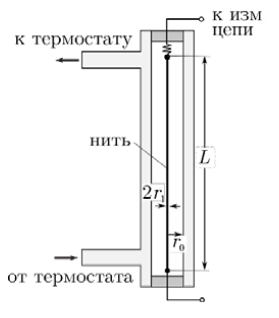
\includegraphics[width=0.3\textwidth]{1.png}
\caption{Схема установки}
\label{ris1}
\end{wrapfigure}

На оси полой цилиндрической трубки с внутреннимдиаметром $2r_0=(1,00\pm0,01)см$ размещена металлическая нить диаметром $2r_1=(0,055\pm0,005)мм$ и длиной $L=(365\pm2)мм$ (материал нити и точные геометрические размеры указаныв техническом описании установки). Полость трубки заполнена воздухом (полость через небольшое отверстие сообщается с атмосферой). Стенки трубки помещены в кожух, через которых пропускается вода из термостата, так что их температура поддерживается постоянной. Для предотвращения конвекции трубка  расположена вертикально.

Металлическая нить служит как источником тепла, так и датчиком температуры (термометром сопротивления). По пропускаемому через нить постоянному току I и напряжению U на ней вычисляется мощность нагрева по закону Джоуля–Ленца:
\begin{equation}\label{4}
	Q = UI,
\end{equation}
и сопротивление по закону Ома:
\begin{equation}\label{5}
	R = \frac{U}{I}.
\end{equation}

Сопротивление нити является однозначной функцией её температуры $R(t)$. Для большинства металлов относительное изменение сопротивления из-за нагрева невелико: приизменении температуры на 1 градус относительное изменение сопротивления нити может составлять приблизительно от 0,2 \% до 0,6\% (в зависимости от её материала).Следовательно, измерение R важно провести с высокой точностью.

\begin{wrapfigure}{r}{0.55\textwidth}
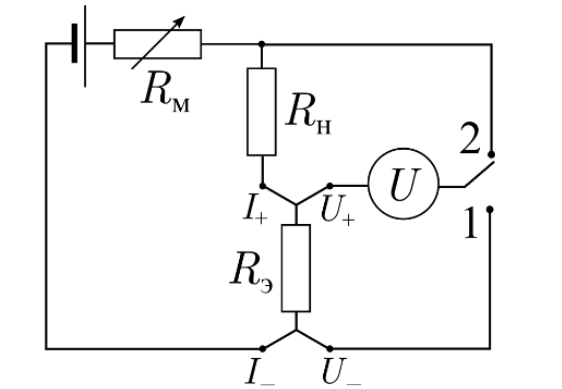
\includegraphics[width=0.5\textwidth]{2.png}
\caption{Электрическая схема измерения сопротивления нити и мощности нагрева}
\label{ris2}
\end{wrapfigure}

Схема предусматривает использование одного вольтметра и эталонного сопротивления $R_э\sim10 \: Ом$, включённого последовательно с нитью. В положении переключателя 2 вольтметр измеряет напряжение на нити, а в положении 1 — напряжениена $R_э$, пропорциональное току через нить. Для исключения влияния контактов и подводящих проводов эталонное сопротивление $R_э$ также   необходимо подключать в цепь по четырёхпроводной схеме.
Ток в цепи в обеих схемах регулируется с помощью реостата или магазина сопротивлений $R_м$, включённого последовательно с источником напряжения.

В исследуемоминтервалетемператур $(20–70~\celsius)$ зависимость сопротивления  от температуры можно с хорошей точностью аппроксимировать линейной функцией:
\begin{equation}\label{6}
	R(t) = R_{273} \cdot (1+\alpha t),
\end{equation}
где t — температурав [$\celsius$], $R_{273}$ — сопротивление нити при температуре $20~\celsius$ и \\ $\alpha = \frac{1}{R_{273}}\frac{dR}{dT}$ — температурный коэффициент сопротивления материала.


\section{Используемое оборудование}

\begin{enumerate}
    \item цилиндрическая колба с натянутой по оси нитью;
    \item термостат;
    \item источник питания постоянного тока;
    \item амперметр, вольтметр (цифровые мультиметры), $\delta_{А} = 0,005~А$;
    \item эталонное сопротивление;
    \item источник постоянного напряжения;
    \item магазин сопротивлений;
\end{enumerate}

\section{Результаты измерений и обработка данных}

Начальные условия:

$\begin{aligned}
& T = 23,1\pm0,1~\celsius
\end{aligned}$\\[0,5 cm]

Проведём предварительные расчёты парметров опыта. Принимая $\Delta{t_{max}} = 10~\celsius$, \\ $\kappa \sim 25~мВт/(м\cdot{K})$, получаем $$Q = 110~мВт; \quad I = \sqrt{\frac{Q}{R}} = 105~мА.$$

Результаты измерений $R(Q)$ представленны в таб. \ref{tab1}-\ref{tab4}.

\begin{table}[h!]
\begin{center}
\begin{tabular}{|c|c|c|c|}
\hline
$Q, 10^{-6}$ Дж & $\sigma_Q, 10^{-6}$ Дж & $R$, Ом & $\sigma_R$, Ом \\ \hline
0,0143 & 0,0001 & 11,00 & 0,01 \\ \hline
0,0174 & 0,0001 & 11,03 & 0,01 \\ \hline
0,0211 & 0,0001 & 11,05 & 0,01 \\ \hline
0,0268 & 0,0001 & 11,06 & 0,01 \\ \hline
0,0348 & 0,0001 & 11,11 & 0,01 \\ \hline
0,0471 & 0,0001 & 11,14 & 0,01 \\ \hline
0,0670 & 0,0001 & 11,16 & 0,01 \\ \hline
\end{tabular}
\end{center}
\caption{$T_1 = 23,1~\celsius$}
\label{tab1}
\end{table} 

\begin{table}[h!]
\begin{center}
\begin{tabular}{|c|c|c|c|}
\hline
$Q, 10^{-6}$ Дж & $\sigma_Q, 10^{-6}$ Дж & $R$, Ом & $\sigma_R$, Ом \\ \hline
0,0149 & 0,0001 & 11,09 & 0,01 \\ \hline
0,0180 & 0,0001 & 11,14 & 0,01 \\ \hline
0,0221 & 0,0001 & 11,14 & 0,01 \\ \hline
0,0280 & 0,0001 & 11,20 & 0,01 \\ \hline
0,0363 & 0,0001 & 11,19 & 0,01 \\ \hline
0,0491 & 0,0001 & 11,22 & 0,01 \\ \hline
0,0703 & 0,0001 & 11,27 & 0,01 \\ \hline
\end{tabular}
\caption{$T_2 = 35~\celsius$}
\label{tab2}
\end{center}
\end{table}

\begin{table}[h!]
\begin{center}
\begin{tabular}{|c|c|c|c|}
\hline
$Q, 10^{-6}$ Дж & $\sigma_Q, 10^{-6}$ Дж & $R$, Ом & $\sigma_R$, Ом \\ \hline
0,0153 & 0,0001 & 11,51 & 0,01 \\ \hline
0,0185 & 0,0001 & 11,52 & 0,01 \\ \hline
0,0229 & 0,0001 & 11,57 & 0,01 \\ \hline
0,0288 & 0,0001 & 11,58 & 0,01 \\ \hline
0,0379 & 0,0001 & 11,67 & 0,01 \\ \hline
0,0507 & 0,0001 & 11,68 & 0,01 \\ \hline
0,0724 & 0,0001 & 11,69 & 0,01 \\ \hline
\end{tabular}
\caption{$T_3 = 45~\celsius$}
\label{tab3}
\end{center}
\end{table}

\newpage

\begin{table}[h!]
\begin{center}
\begin{tabular}{|c|c|c|c|}
\hline
$Q, 10^{-6}$ Дж & $\sigma_Q, 10^{-6}$ Дж & $R$, Ом & $\sigma_R$, Ом \\ \hline
0,0206 & 0,0001 & 12,65 & 0,01 \\ \hline
0,0254 & 0,0001 & 12,76 & 0,01 \\ \hline
0,0321 & 0,0001 & 12,77 & 0,01 \\ \hline
0,0419 & 0,0001 & 12,77 & 0,01 \\ \hline
0,0569 & 0,0001 & 12,79 & 0,01 \\ \hline
0,0819 & 0,0001 & 12,80 & 0,01 \\ \hline
0,1280 & 0,0001 & 12,80 & 0,01 \\ \hline
\end{tabular}
\caption{$T_4 = 70~\celsius$}
\label{tab4}
\end{center}
\end{table}

Полученная зависимость $R$ от $Q$ представленна на рис. \ref{ris3}.
\begin{figure}[h!]
\begin{flushleft}
    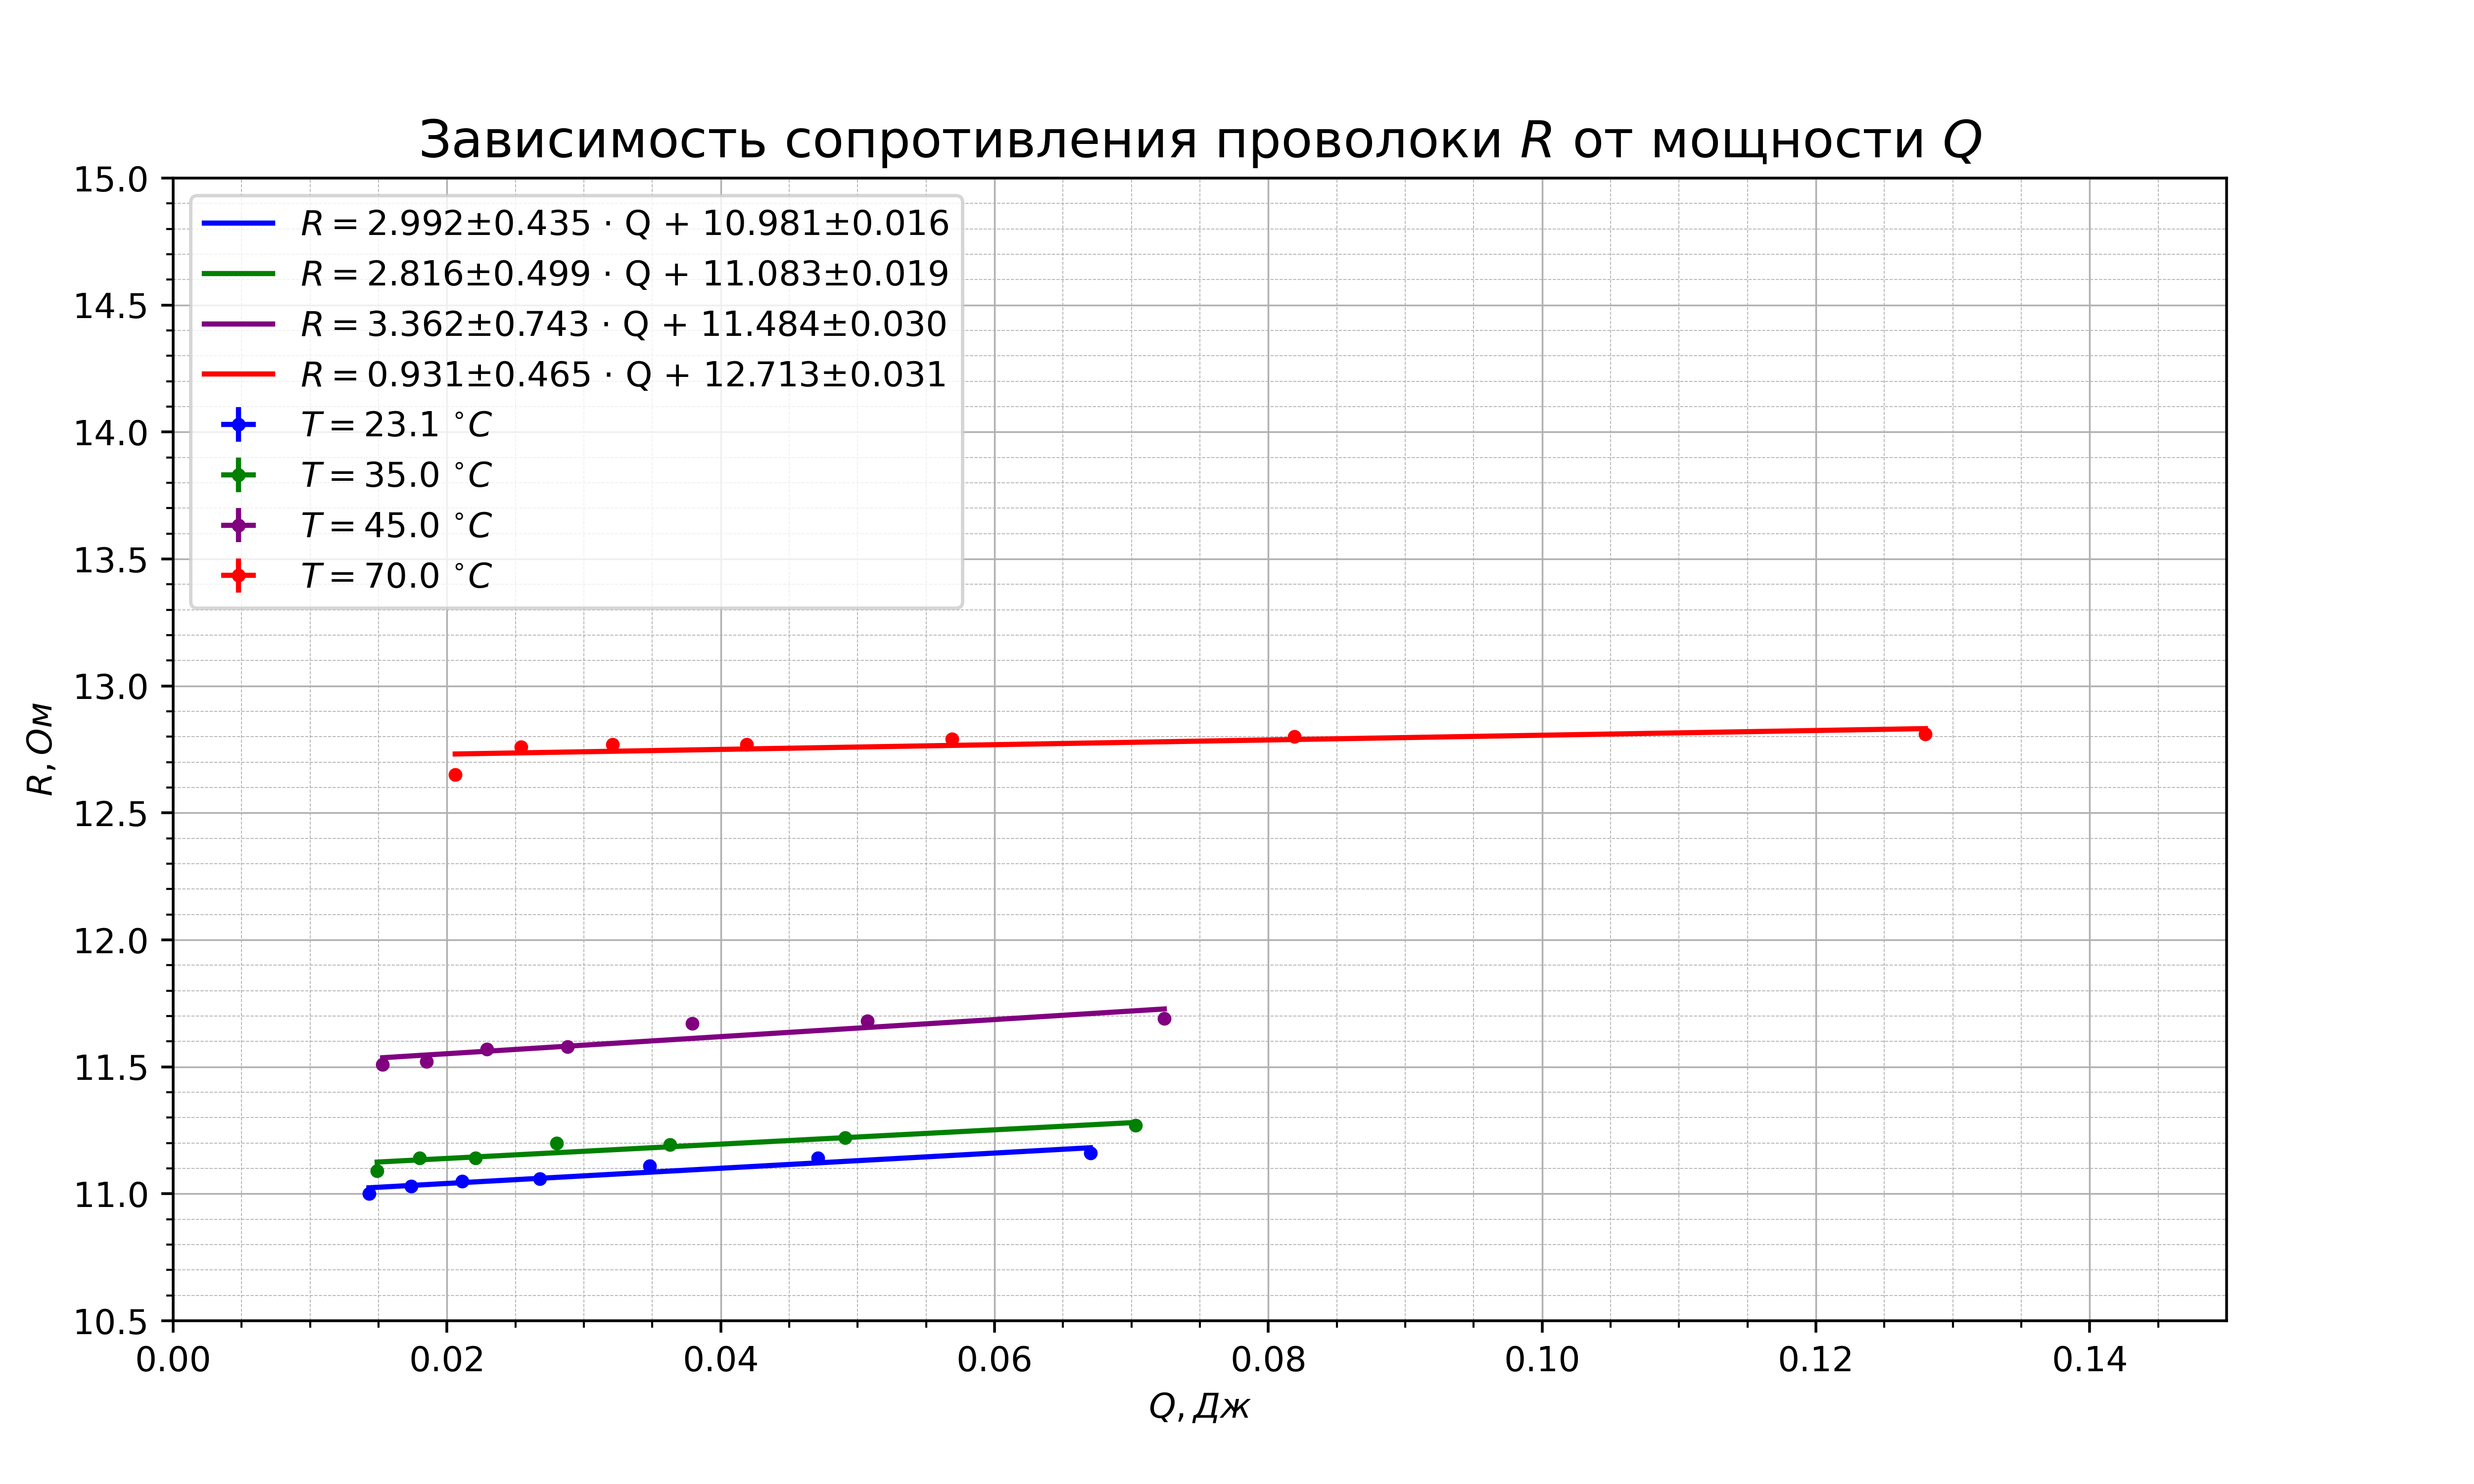
\includegraphics[scale=0.75]{2.2.3_1.png}
\end{flushleft}
\caption{}
\label{ris3}
\end{figure}

Полученная зависимость $R_0$ от $T$ представленна на рис. \ref{ris4}.
\begin{figure}[h!]
\begin{flushleft}
    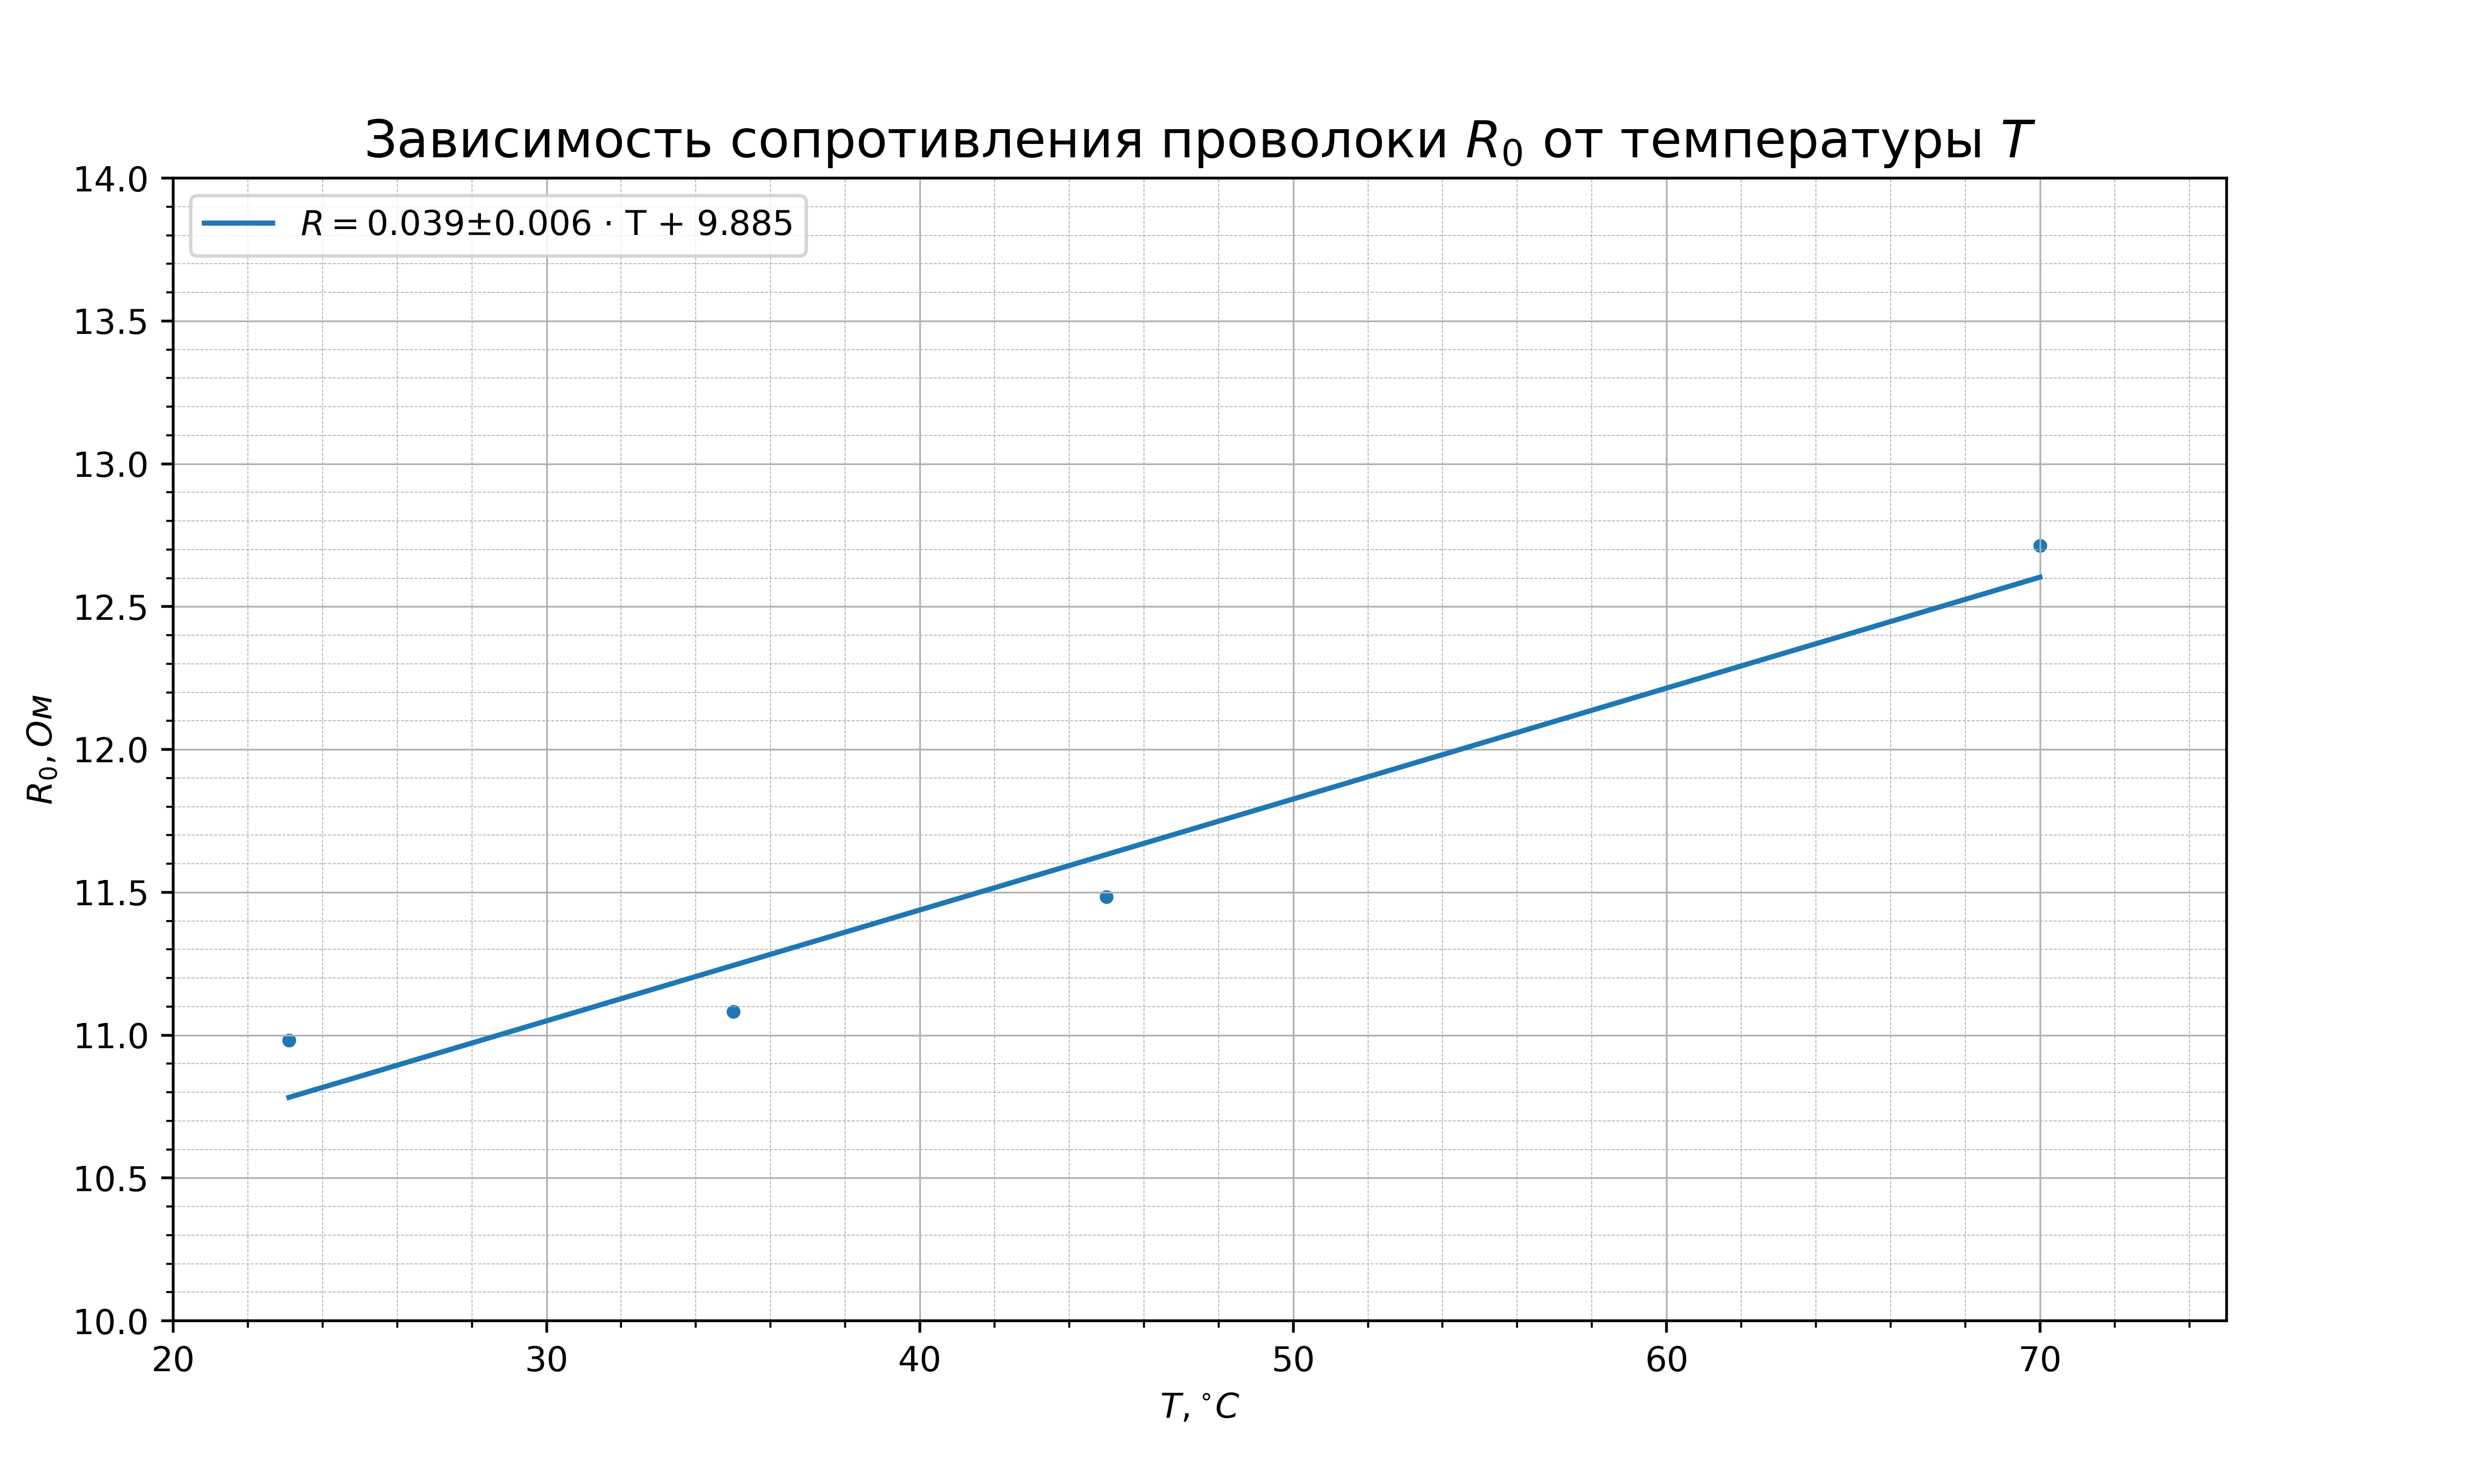
\includegraphics[scale=0.75]{2.2.3_2.png}
\end{flushleft}
\caption{}
\label{ris4}
\end{figure}

Полученное значение температурного коэффициента сопротивления
$$\boxed{\alpha = \frac{1}{R_{273}}\frac{dR}{dT} = 0,0047\pm0,0008~K^{-1}}.$$

Полученные коэффициенты теплопроводности $\kappa$ представленны в таб. \ref{tab5}.

\newpage

\begin{table}[h!]
\begin{center}
\begin{tabular}{|c|c|c|c|c|}
\hline 
$T,~\celsius$ & $dR/dT$ & $dR/dQ$ & $dQ/\Delta{T}$ & $\kappa,~Вт/(K \cdot м) $ \\ 
\hline 
23,1 & $0,039\pm0,006$ & $2,992\pm0,435$ & $0,013\pm0,003$ & $0,029\pm0,006$ \\ 
\hline 
35 & $0,039\pm0,006$ & $2,816\pm0,499$ & $0,014\pm0,003$ & $0,031\pm0,007$ \\ 
\hline 
45 & $0,039\pm0,006$ & $3,362\pm0,743$ & $0,012\pm0,003$ & $0,026\pm0,007$ \\ 
\hline 
70 & $0,039\pm0,006$ & $0,931\pm0,465$ & $0,022\pm0,075$ & $0,049\pm0,015$ \\ 
\hline 
\end{tabular} 
\caption{Результаты вычислений}
\label{tab5}
\end{center}
\end{table}

Полученная зависимость $\kappa$ от $T$ представленна на рис. \ref{ris5}.
\begin{figure}[h!]
\begin{flushleft}
    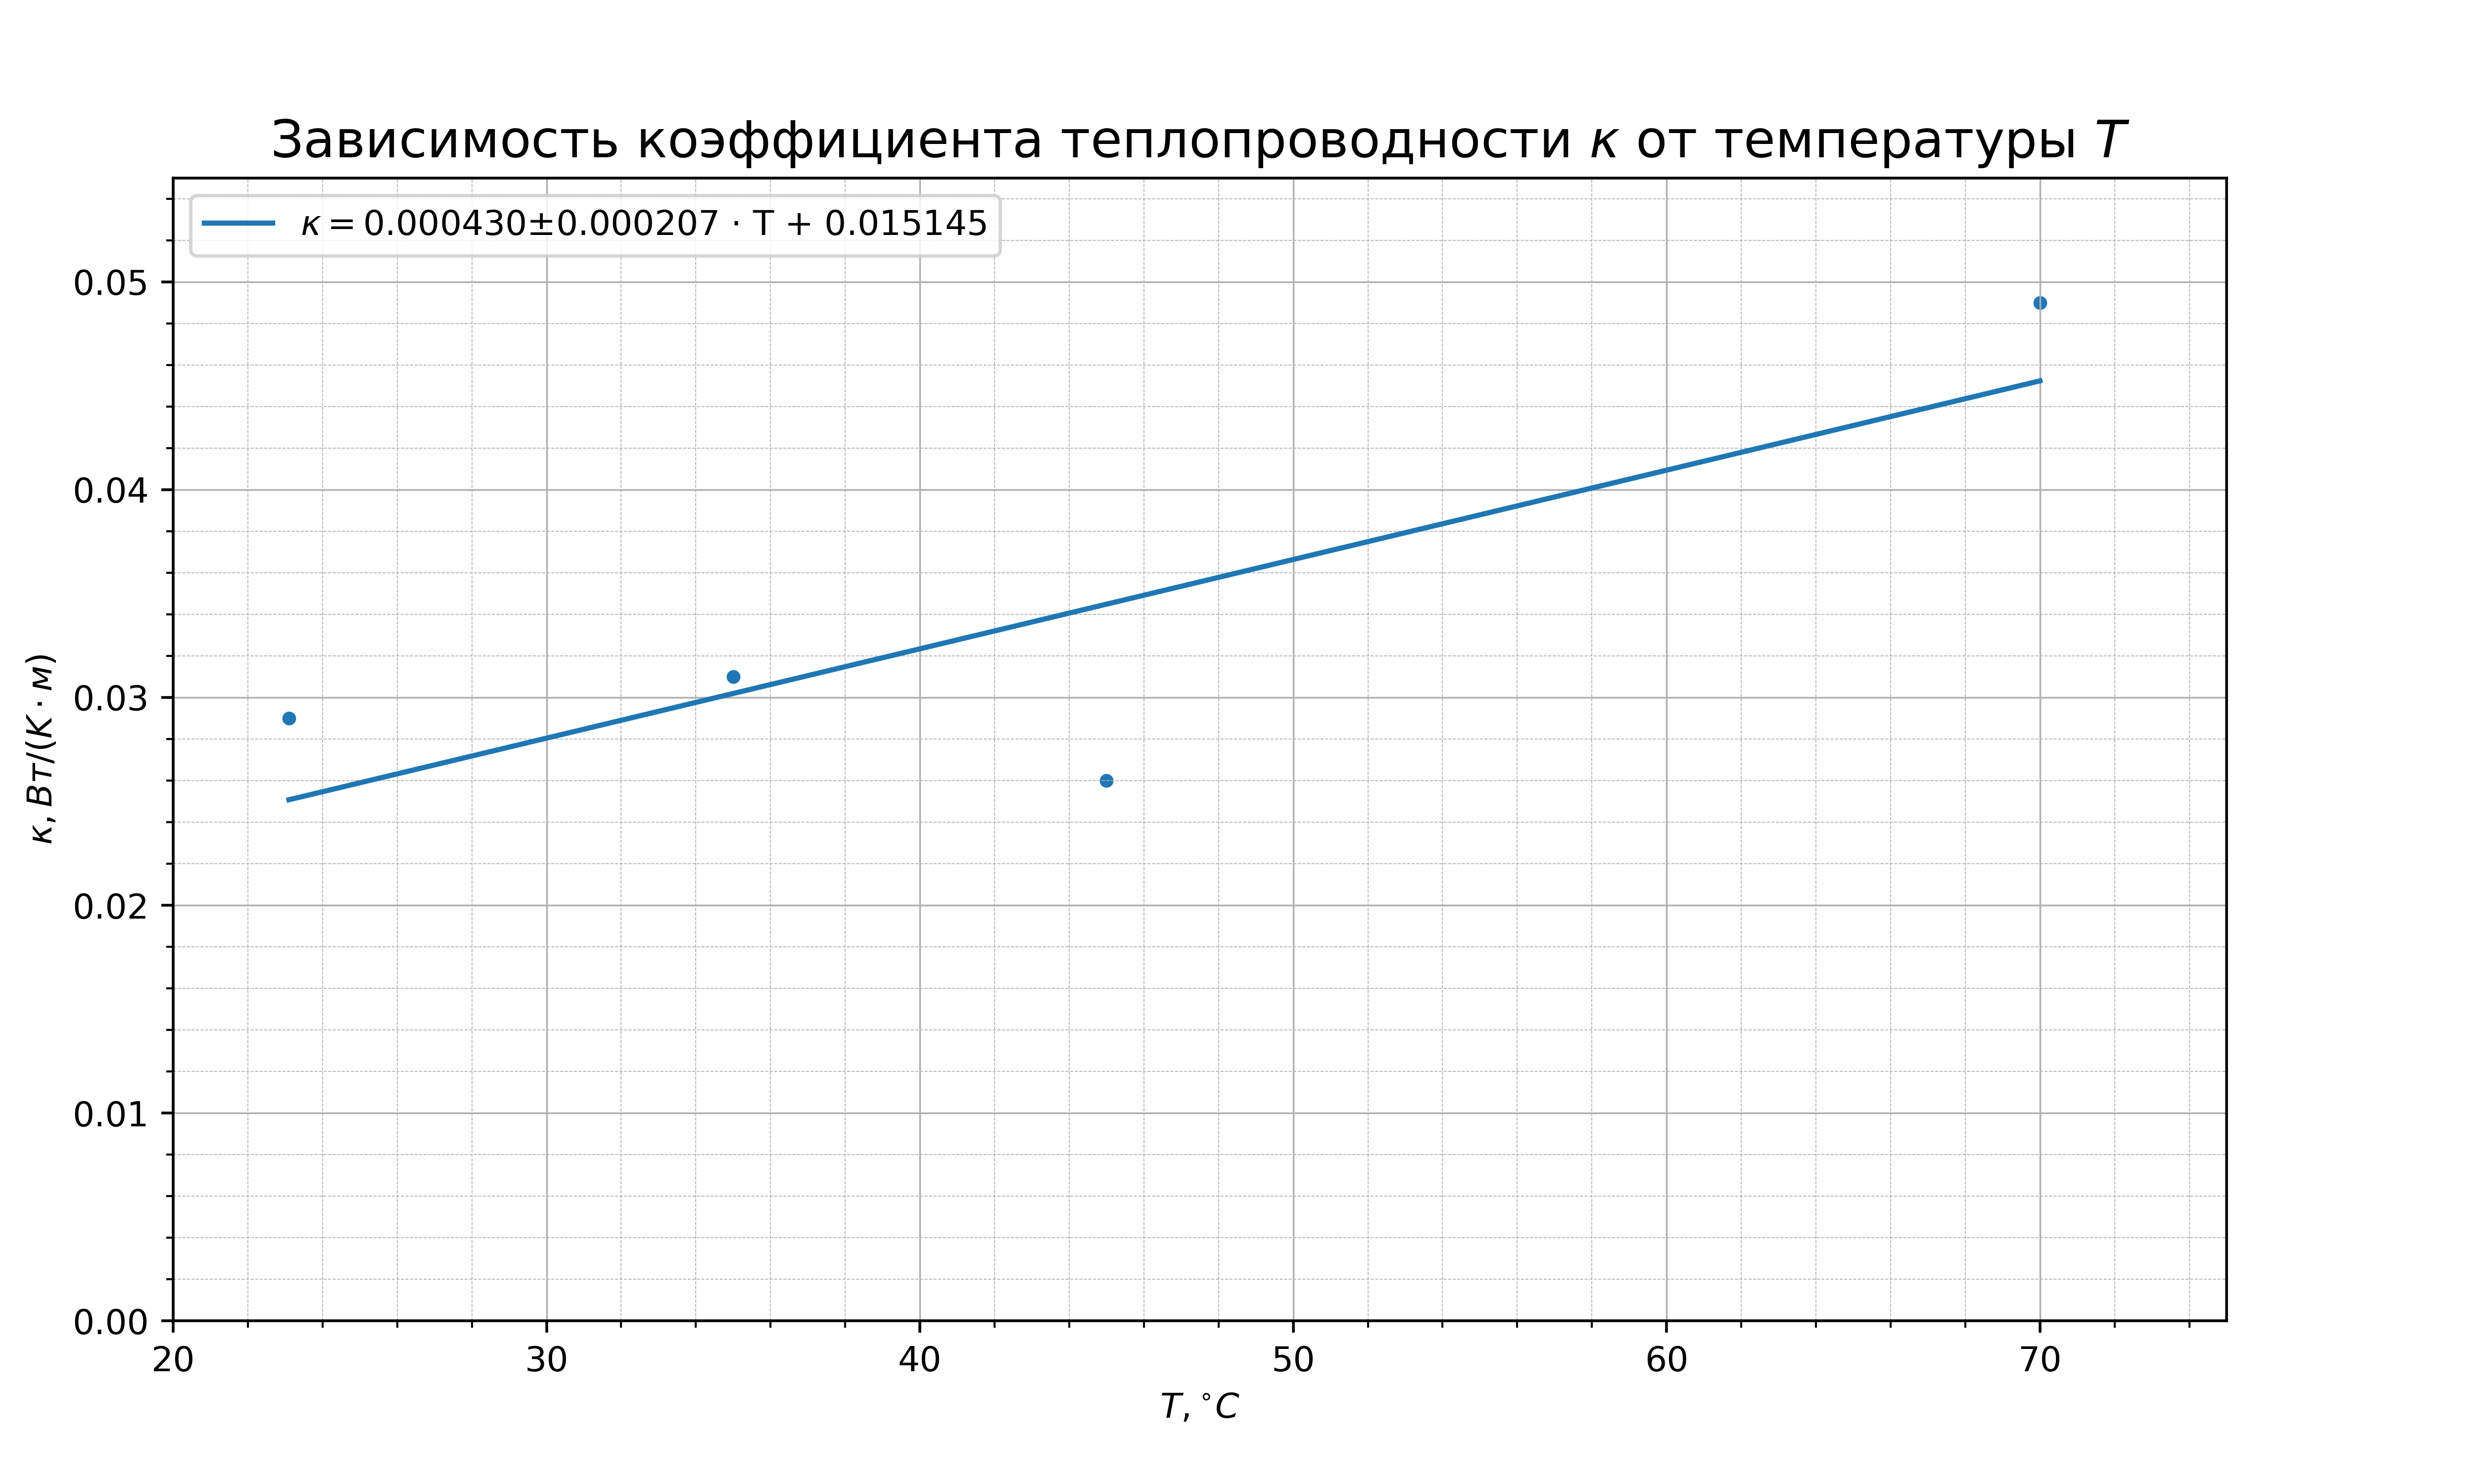
\includegraphics[scale=0.75]{2.2.3_3.png}
\end{flushleft}
\caption{}
\label{ris5}
\end{figure}

Полученная зависимость $\ln{\kappa}$ от $\ln{T}$ представленна на рис. \ref{ris6}.
\begin{figure}[h!]
\begin{flushleft}
    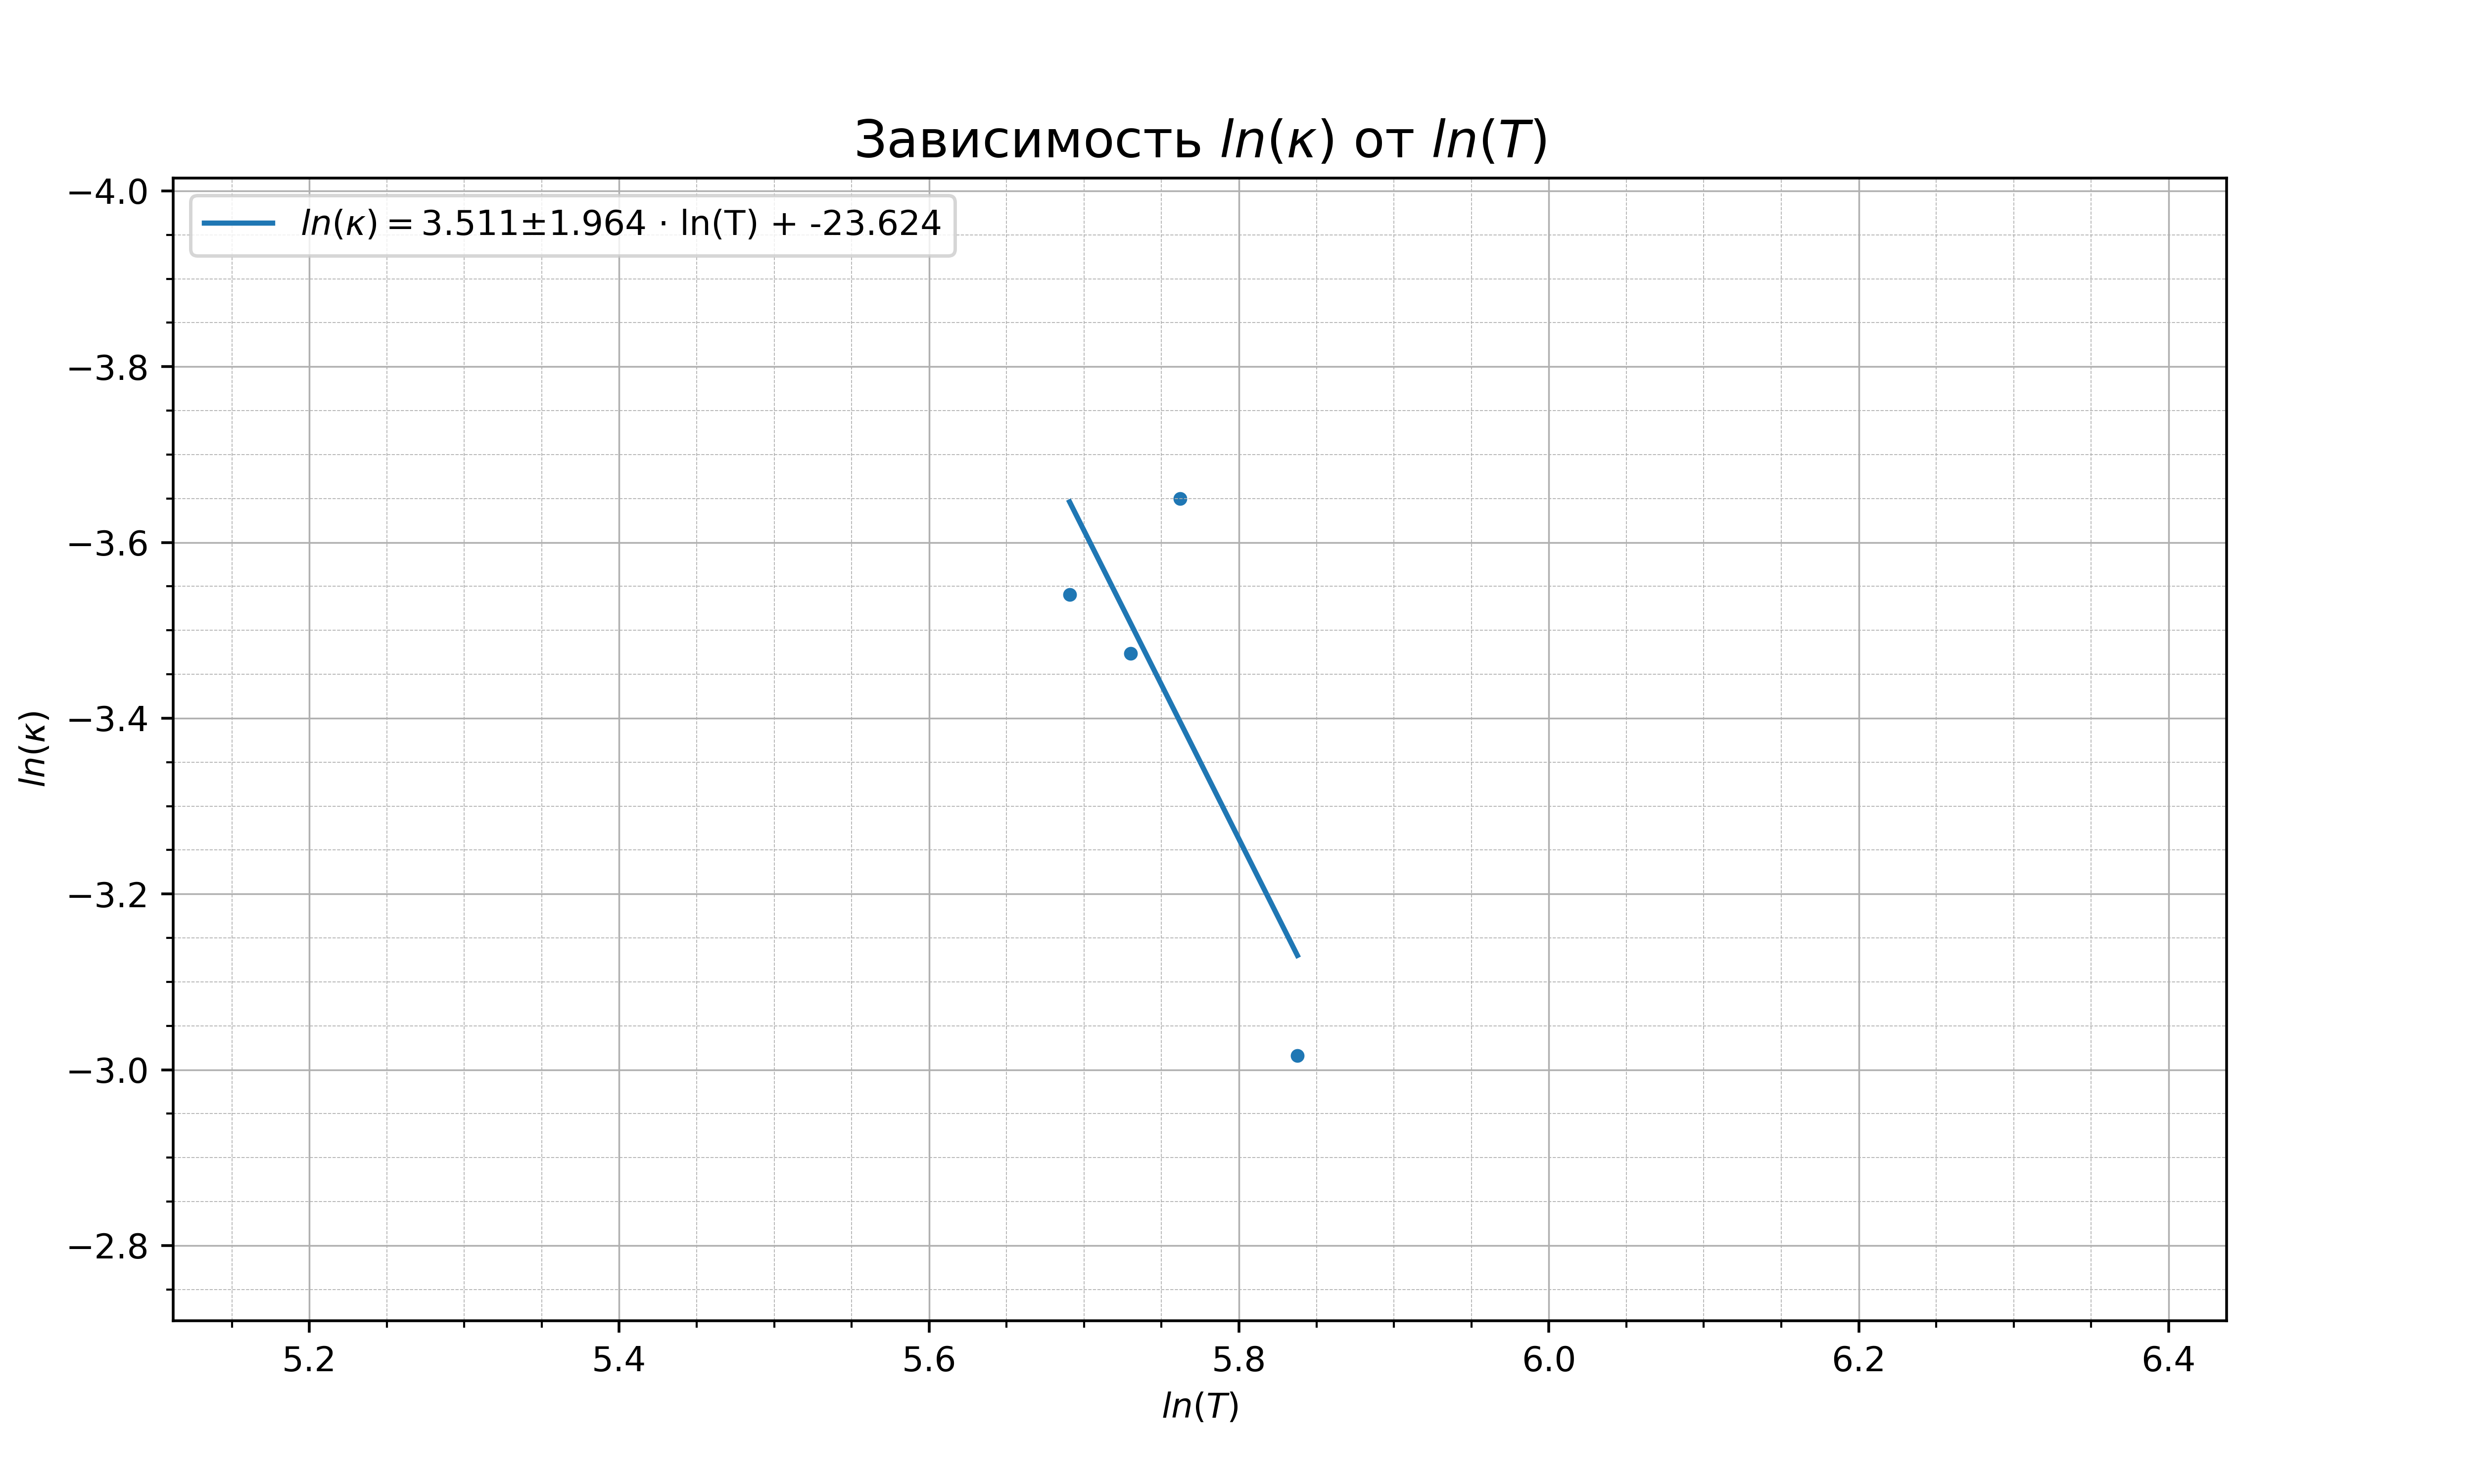
\includegraphics[scale=0.75]{2.2.3_4.png}
\end{flushleft}
\caption{}
\label{ris6}
\end{figure}

Полученное значение $$\boxed{\beta = 3,511\pm1,964}.$$

\newpage

\section{Обсуждение результатов и выводы}

В данной работе исследовалась зависимость сопротивления проволоки от мощности выделяющегося на ней тепла. По результатам измерений для каждой температуры определялся коэффициент теплопроводности воздуха. Полученная зависимость представленна на рис. \ref{ris5}. Полученные значения для всех температур, кроме $70~\celsius$, согласуются с табличными данными -- $\kappa = 0,025\div0,030~Вт/(K \cdot м)$.
Использованный в работе метод измерений позволяет достичь относительной точности результатов в 20\%. Основной вклад в погрешность вносит погрешность определения коэффициентов линейной зависимости.

Также в данной работе был определён температурный коэффициент сопротивления молибдена:
$$\boxed{\alpha = \frac{1}{R_{273}}\frac{dR}{dT} = 0,0047\pm0,0008~K^{-1}}.$$
Табличное значение для данного коэффициента -- $0,0049~K^{-1}$, что согласуется с полученным результатом.

В простейшей модели твёрдых шариков коэффициент теплопроводности пропорционален корню абсолютной температруы $\kappa \varpropto T^{\frac{1}{2}}$. Эксперементальное значение показателя степени $$\boxed{\beta = 3,511\pm1,964},$$ что слабо согласуется с теорией. Во-первых, это может быть связано с неучтенными тепловыми потерями через основания цилиндра. Во-вторых, количество экспериментальных точек достаточно мало. В-третьих, при выводе формулы \eqref{3} пренебрегалось зависимостью теплопроводности от температуры, поэтому она справедлива только при $\Delta T \ll T$. И наконец, возникновение термо-ЭДС повлияло на точность вольтметра. Для получения более точного результата необходимо увеличить диапазон рабочих температур, количество экспериментальных точек и уменьшить шаг изменения температуры.

\end{document}